% Presentazione seminario multilanguage word-based alignment Lione 26-11-2019

\documentclass{beamer}
    
%    \usepackage[english]{babel}
    %\usepackage[latin1]{inputenc}
    %\usepackage[T1]{fontenc}

\mode<presentation>{
  \setbeamertemplate{background canvas}[vertical shading]
  \usetheme{Berkeley}
  \useoutertheme{himinfolines}
}
  
\usepackage{ucs}
\usepackage[utf8]{inputenc}
\usepackage[english,polutonikogreek,italian,UKenglish,british]{babel}
\usepackage{graphicx}
\usepackage{colortbl}
\usepackage{multicol}
\usepackage{ulem}
\usepackage{verbatim}
\usepackage{alltt}
\usepackage{ccicons}
\usepackage{MnSymbol,wasysym}
\usepackage{tikzsymbols}
\usepackage{textcomp}
\usepackage{xmpincl}

\usepackage{parskip}
\setcounter{nframes}{100}
\setcounter{nframe}{1}
\setbeamercovered{dynamic}
\newenvironment{grcenv}{\begin{otherlanguage}{greek}}{\end{otherlanguage}}
\newcommand{\g}[1]{\textgreek{#1}}
\definecolor{darkgreen}{rgb}{0,0.5,0}
\definecolor{darkblue}{rgb}{0,0,0.5}
\definecolor{grey}{rgb}{0.5,0.5,0.5}
\setcounter{tocdepth}{5}

\makeatletter

\makeatother
%\includexmp{LicencesAndLicensing}

%frame00 metadata
	\title{Dalla recensio all'emendatio digitale}
	\author[A.M. Del Grosso]{Angelo Mario Del Grosso}
	%\institute{}
	%\institute{\texttt{angelo.delgrosso@ilc.cnr.it} \\\bigskip\textit{CNR-ILC-LicoLab} \\\bigskip\url{http://licolab.ilc.cnr.it/}}
    \institute{\texttt{angelo.delgrosso@ilc.cnr.it} \\\bigskip\textbf{Methodology}}
    \date{Istituto di Linguistica Computazionale ``A. Zampolli'', \today}
    \AtBeginSection[]{
    \begin{frame}<beamer>
    \addtocounter{nframe}{1}
    \footnotesize
    \frametitle{Progress status}
    \tableofcontents[currentsection,hideothersubsections]
    \end{frame}
    }

\begin{document}

\begin{frame}
	\maketitle
\end{frame}

\begin{frame}
	\frametitle{Outline}
	\tableofcontents
\end{frame}

\section{Self Introduction}

\begin{frame}
	\frametitle{What is my work about}
	\addtocounter{nframe}{1}

	\begin{block}{My interests}
		\begin{center}
			I am a computer engineer involed in computational philology
		\end{center}
	\end{block}

	\begin{center}
		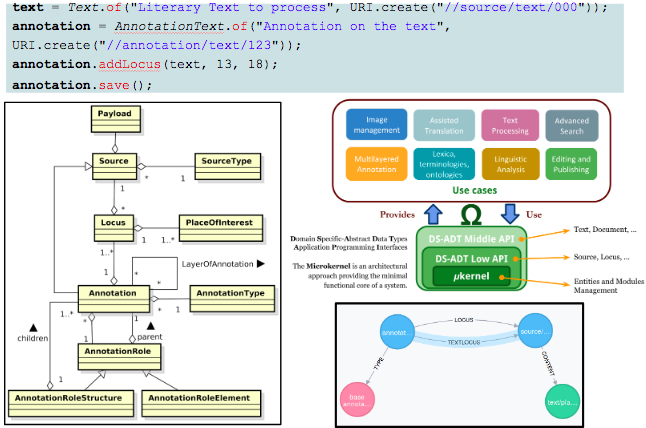
\includegraphics[width=.7\textwidth]{imgs/InfrastructureForTextualScholarship.png}
	\end{center}

\end{frame}

\begin{frame}
	\frametitle{DH projects}
	\addtocounter{nframe}{1}

	\begin{itemize}
		\item 
		\item 
		\item 
		\item 
		\item 
		\item 
	\end{itemize}

\end{frame}

\section{Introduction}
\begin{frame}
    \frametitle{Intro}
    \framesubtitle{Getting started}
    \addtocounter{nframe}{1}
    
    \begin{block}{Main Discipline}
    \end{block}

    \begin{block}{Main Goal}
    \end{block}

\end{frame}

\begin{frame}
    \frametitle{Introduction}
    \addtocounter{nframe}{1}
    
    \begin{center}
        \includegraphics[width=.95\textwidth]{imgs/1.png}
    \end{center}

\end{frame}

 


\section{Project}
\input{includes/section1.tex}

\section{Other}
\input{includes/section2.tex}

\section{Next}
\input{includes/section3.tex}

\section{Conclusions}

% \begin{frame}
% 	\frametitle{Conclusion and Further Work}
% 	\addtocounter{nframe}{1}
% 	\begin{block}{Conclusion}
		
% 	\end{block}
% 	\begin{block}{Conclusion}
		
% 	\end{block}
% \end{frame}


% \begin{frame}
% 	\frametitle{Conclusion and Further Work}
% 	\addtocounter{nframe}{1}
% 	\begin{block}{Conclusion}
% 		\begin{itemize}
% 			\item 
% 			\item 
% 		\end{itemize}
% 	\end{block}
% \end{frame}


% \begin{frame}
% 	\frametitle{Conclusion and Further Work}
% 	\addtocounter{nframe}{1}
% 	\begin{block}{Conclusion:}
% 		\begin{itemize}
% 			\item<1-> 
% 			\item<2-> 
% 			\item<3-> 
% 			\item<4-> 
% 		\end{itemize}
% 	\end{block}
% \end{frame}

%% lavori futuri %%


\begin{frame}
	\frametitle{Conclusion and Further Work}
	\addtocounter{nframe}{1}
	\begin{block}{FINE DEL SEMINARIO!!}
		\begin{center}
			Grazie per la vostra paziente attenzione
		\end{center}
		\begin{center}
			\textbf{Se ci sono domande..}
		\end{center}
	\end{block}
\end{frame}



\section{References}

%bibliografia
\begin{frame}
    \frametitle{References}
    \addtocounter{nframe}{1}
    \begin{thebibliography}{10}
    \end{thebibliography}

\end{frame}

\begin{frame}
    \frametitle{References}
    \addtocounter{nframe}{1}
    \begin{thebibliography}{10}
    \end{thebibliography}

\end{frame}


\end{document}